\begin{landscape}
	\subsubsection{Poziom 1}
		\begin{figure}[H]
			\centering
			\centerline{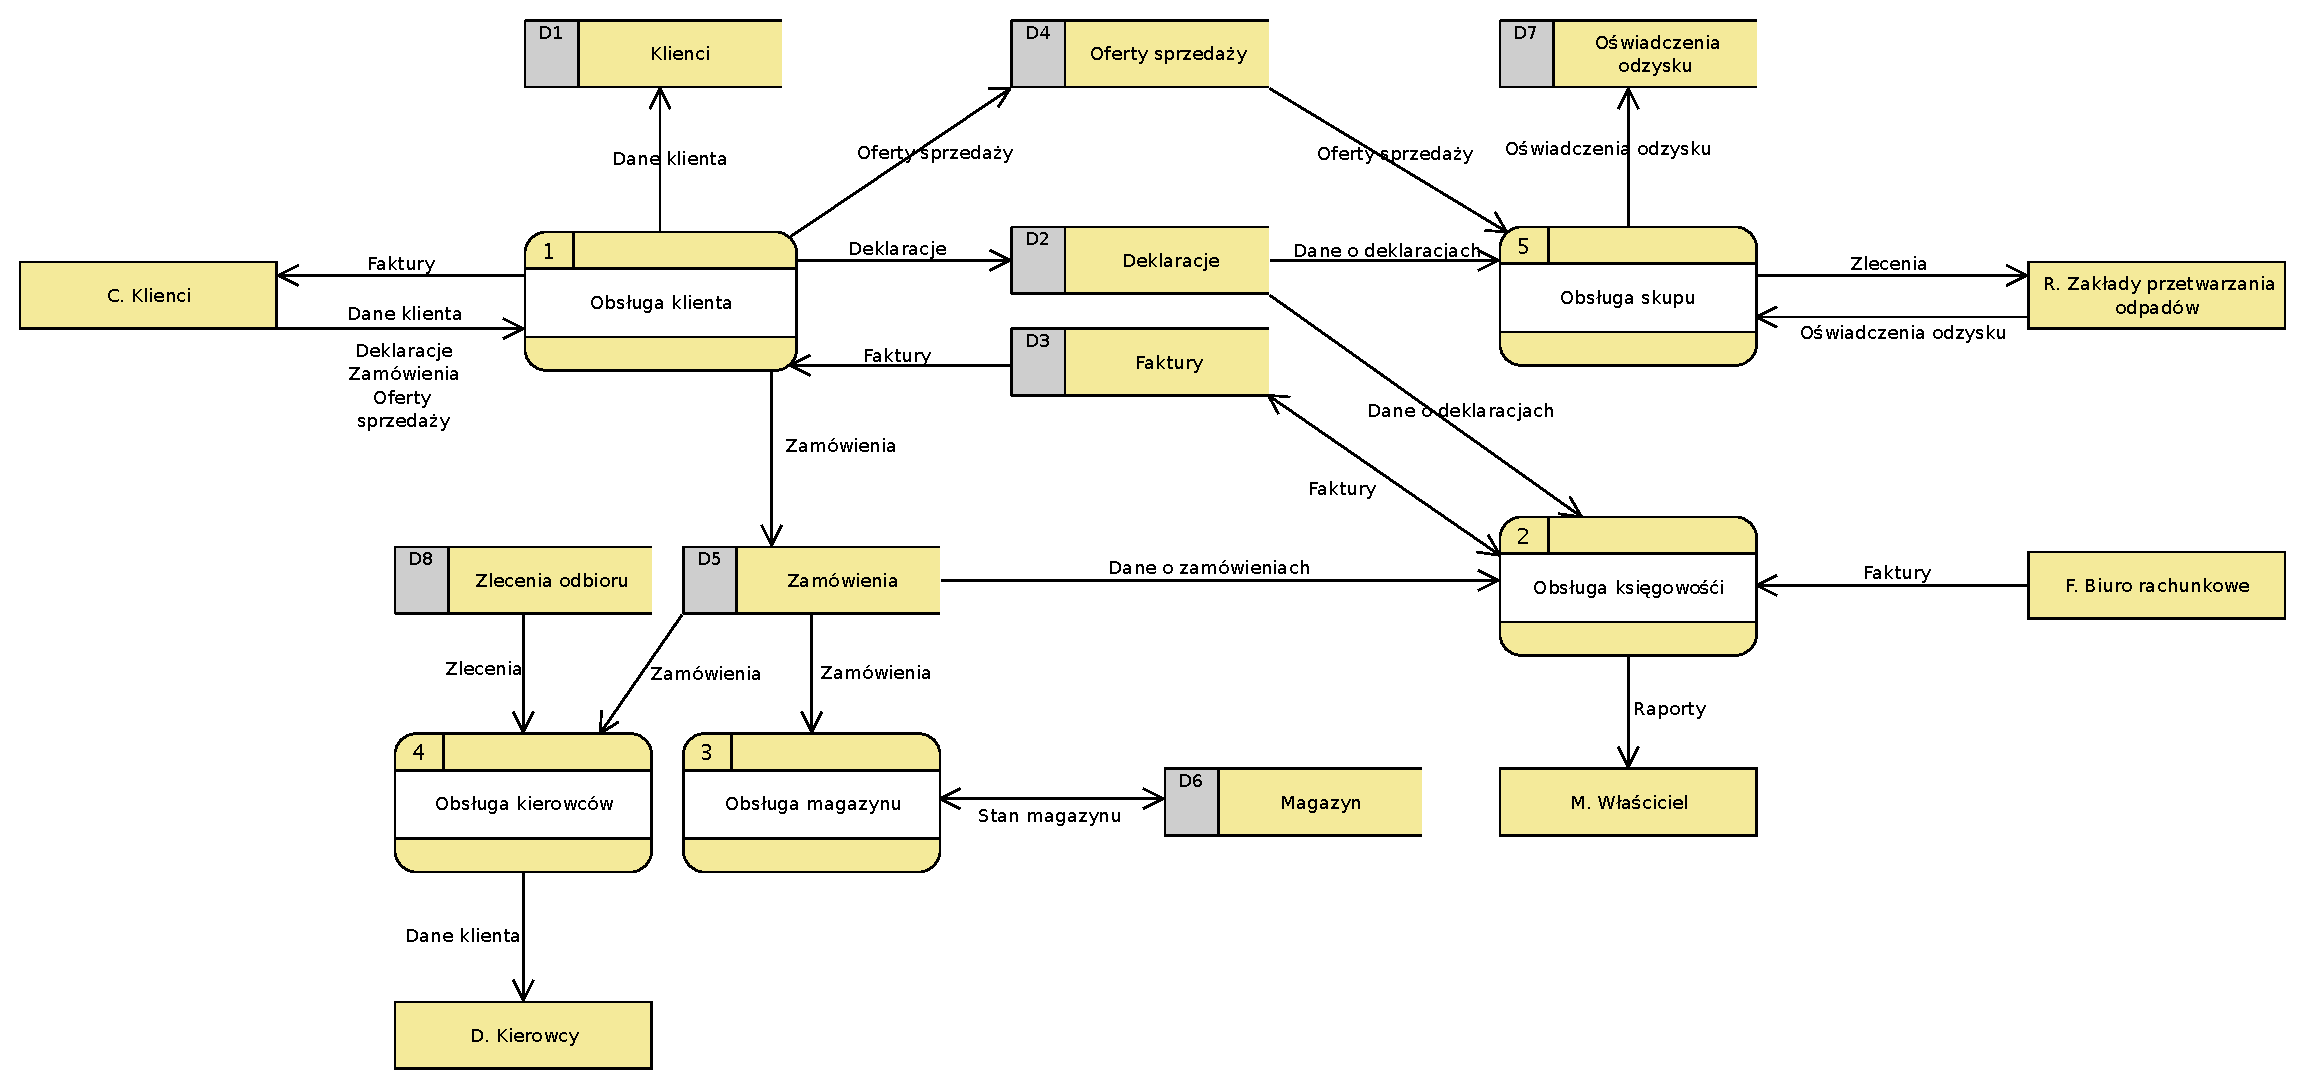
\includegraphics[width=29cm]{img/DFD/1-level.eps}}
		\end{figure}
\end{landscape}

	%DFD1
	\textbf{Opis}\\
	Digram pokazuje wyodrębnienie podsystemów, które są przedstawione bardziej szczegółowo na kolejnych diagramach.

	

\subsubsection{Poziom 2}

	\begin{figure}[H]
		\centering
		\centerline{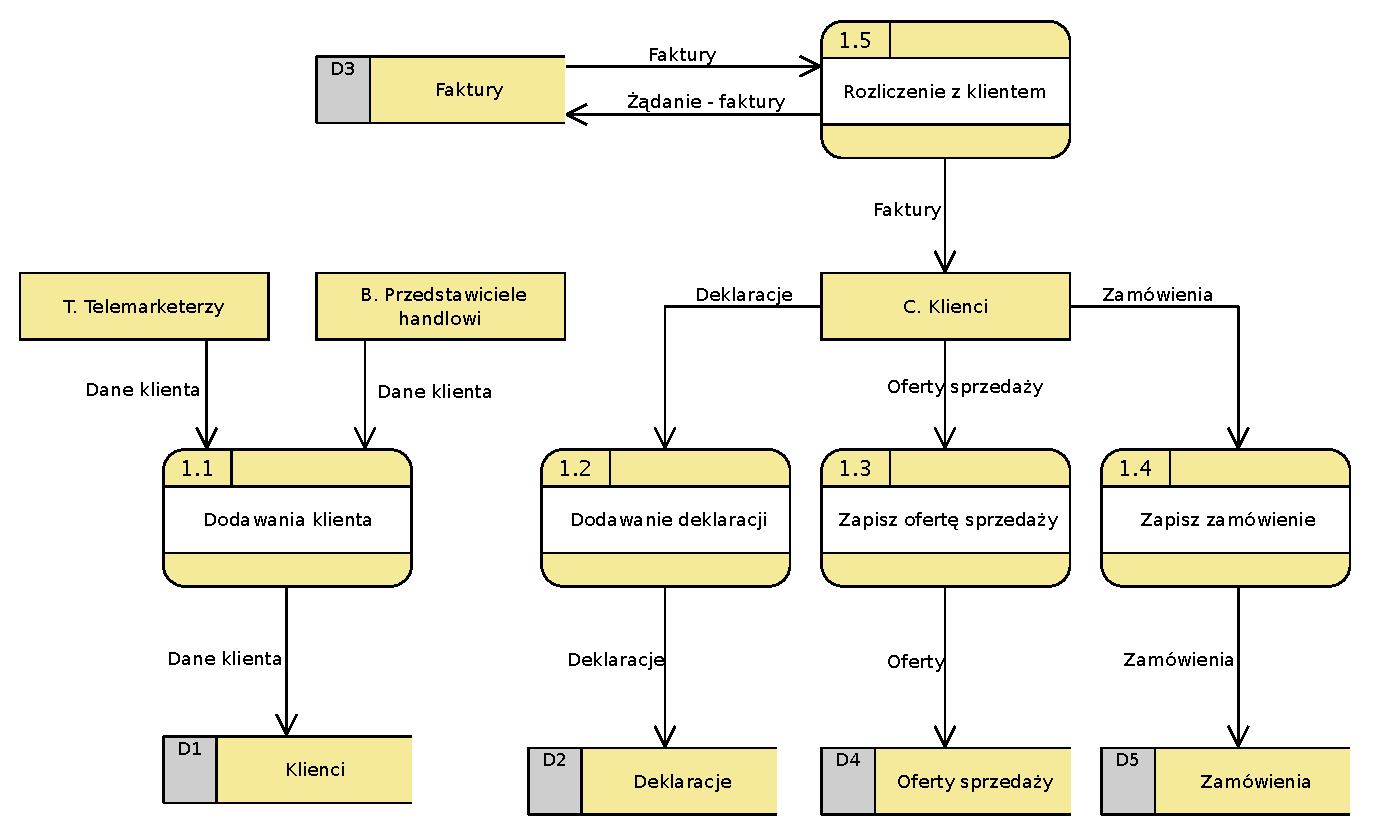
\includegraphics[width=1.2\textwidth]{img/DFD/2-level-klient.eps}}
		\caption{Obsługa klienta}
	\end{figure}

	%DFD2 - Obsługa magazynu
	\begin{figure}[H]
		\centering
		\centerline{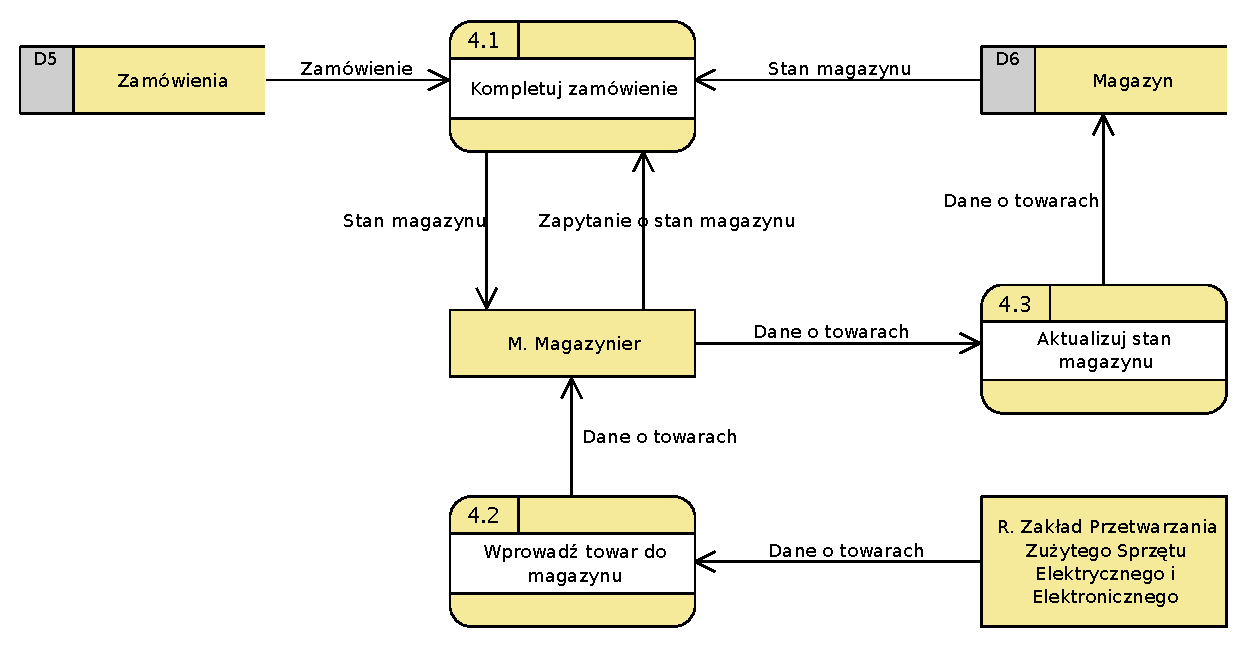
\includegraphics[width=1.1\textwidth]{img/DFD/2-level-magazyn.eps}}
		\caption{Obsługa magazynu}
	\end{figure}

	\textbf{Opis} \\
	\underline{3.1 Kompletuj zamówienie}\\
	Magazynier pyta o stan magazynu, aby sprawdzić, czy może skompletować zamówienie.
	\textbf{Strumień wejściowy} zapytanie o stan magazynu, zamówienie\\
	\textbf{Strumień wyjściowy} aktualny stan magazynu\\

	\underline{3.2 Aktualizuj stan magazynu}\\ 
	Stan magazynu jest aktualizowany na podstawie ilości produktów dostarczanych lub odbieranych.\\	
	\textbf{Strumień wejściowy} Produkty przyjmawane do magazynu, produkty wydawane przez magazyn.\\
	\textbf{Strumień wyjściowy} Produkty przyjmawane do magazynu, produkty wydawane przez magazyn.\\
	\underline{3.3 Wprowadź towar do magazynu}\\
	Towar zostaje przywieziony przez kierowcę z Zakładu Przetwarzania Zużytego Sprzętu Elektrycznego i Elektronicznego, informacje o jego ilości są zapisywane do systemu.\\
	\textbf{Strumień wejściowy} Dane o przywiezionych towarach\\
	\textbf{Strumień wyjściowy} Dane o przywiezionych towarach

	\begin{figure}[H]
		\centering
		\centerline{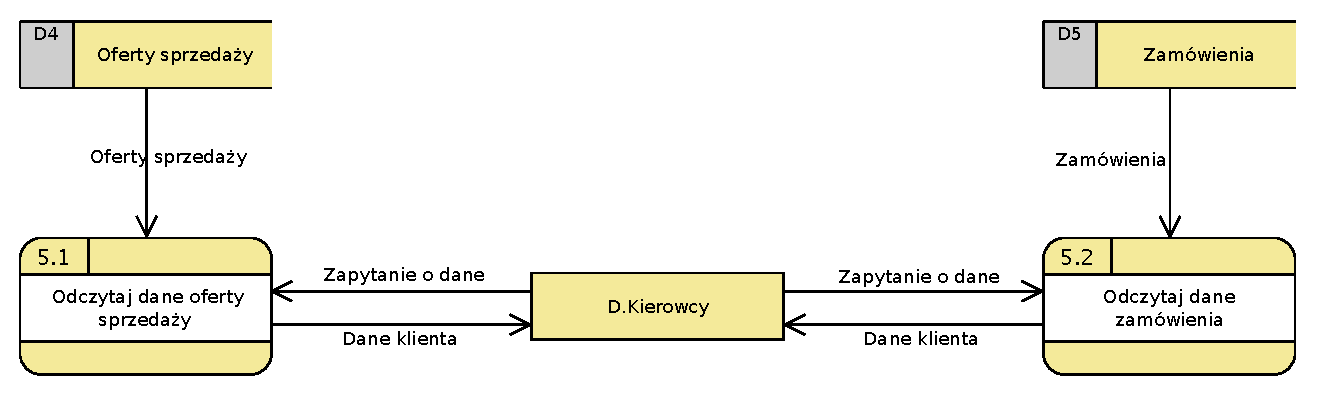
\includegraphics[width=1.1\textwidth]{img/DFD/2-level-kierowcy.eps}}
		\caption{Obsługa kierowców}
	\end{figure}

	\begin{figure}[H]
		\centering
		\centerline{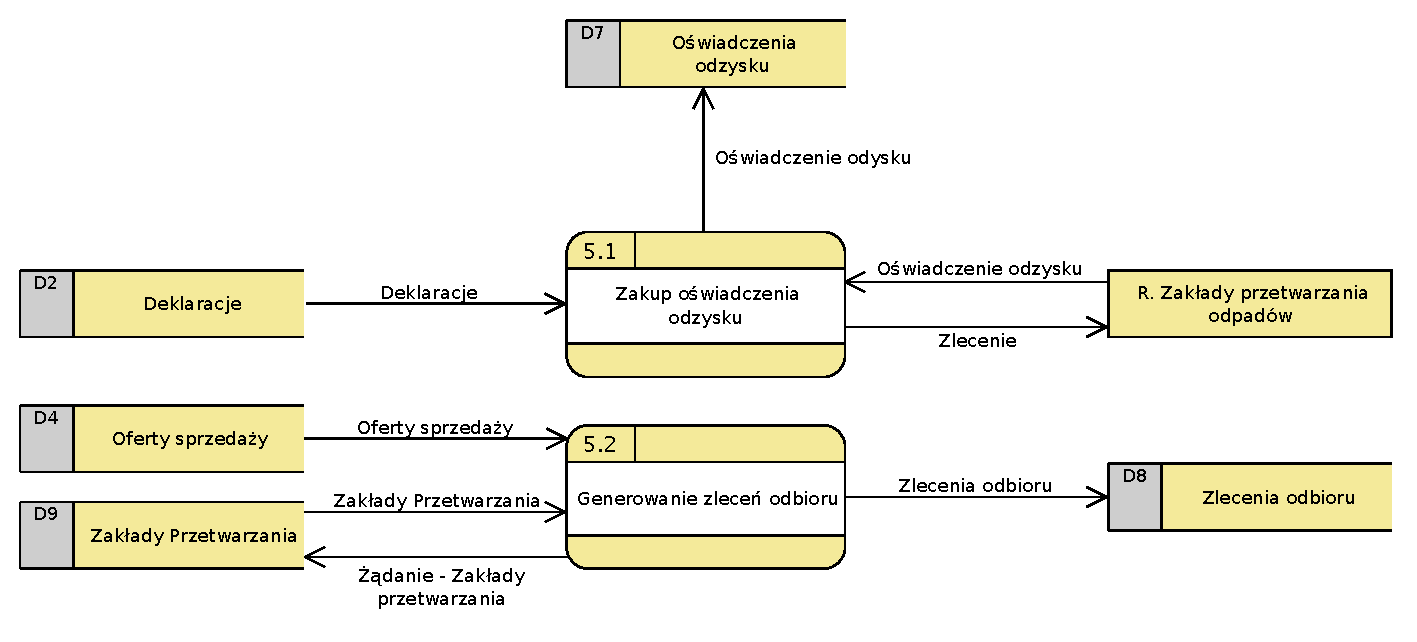
\includegraphics[width=1.1\textwidth]{img/DFD/2-level-skup.eps}}
		\caption{Obsługa skupu}
	\end{figure}

	\begin{figure}[H]
		\centering
		\centerline{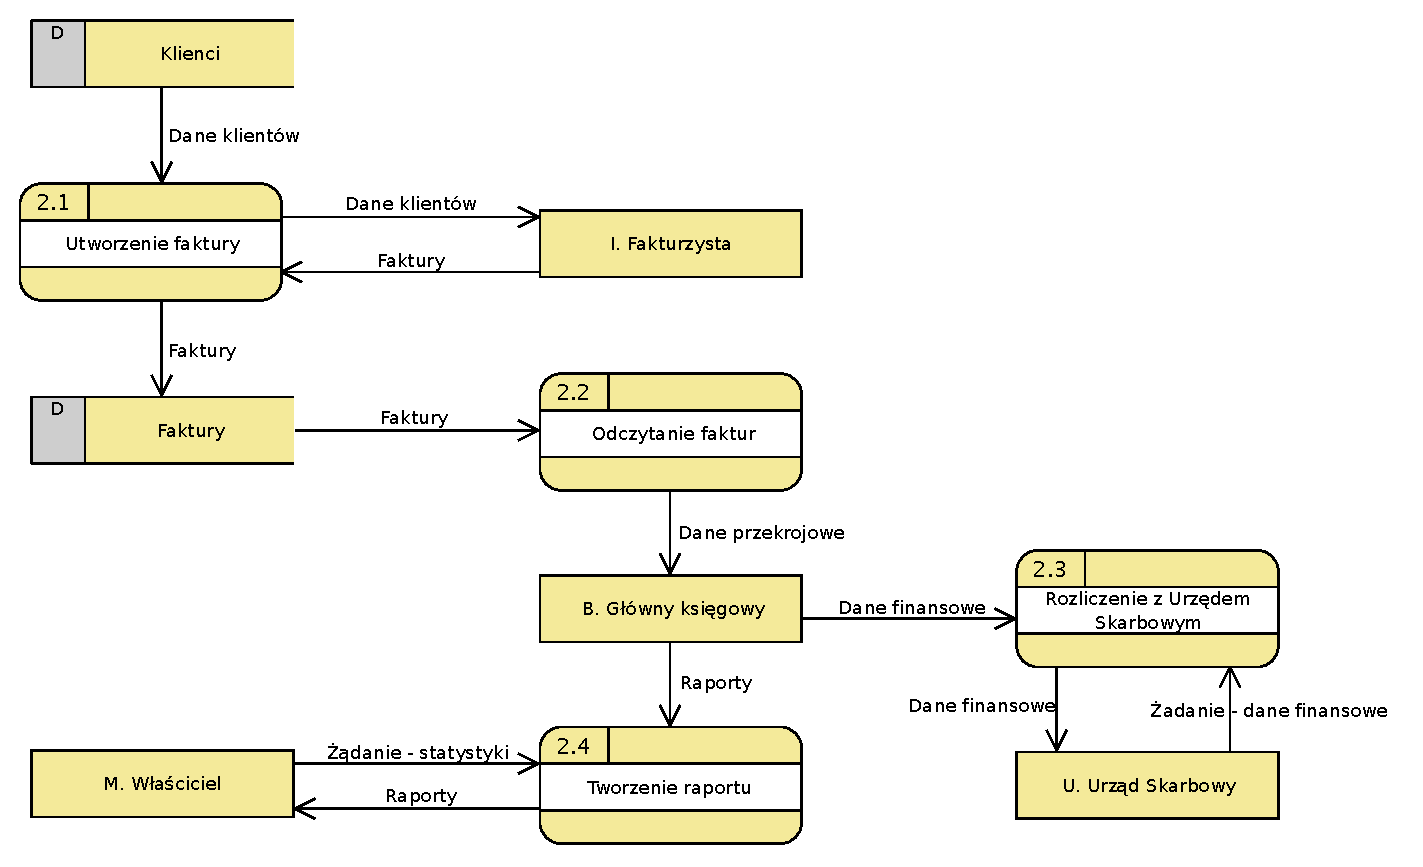
\includegraphics[width=1.1\textwidth]{img/DFD/2-level-ksiegowosc.eps}}
		\caption{Obsługa księgowości}
	\end{figure}